\subsubsection{Name}

ResizeAb -- Modifies the abutment box of the current cell

\subsubsection{Synopsys}

\begin{verbatim}
ResizeAb ( dx1, dy1, dx2, dy2 )
\end{verbatim}

\subsubsection{Description}

This function modifies the abutment box of the current cell.\\
\indent The coordinates of the abutment box are the coordinates of the envelop of the abutment boxes of each instance plus the delta values given as argument.\\

\indent Note that one can not call this function in order to create the abutment box. This fonction only modifies the already created abutment box.
    
\subsubsection{Parameters}

\begin{itemize}
    \item \verb-(dx1, dy1)- : Values to be substracted to the lower left corner of the previous abutment box.
    \item \verb-(dx2, dy2)- : Values to be added to the upper right corner of the previous abutment box.
\end{itemize}

\indent The Values are used as follow :
\begin{figure}[h!]
\centering
\latexhtml{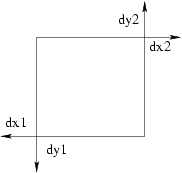
\includegraphics[width=.3\textwidth]{./images/resizeAb}}
          {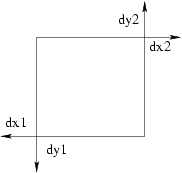
\includegraphics[width=.3\textwidth]{./images/resizeAb.png}}
\end{figure}
      
\subsubsection{Example}

\begin{verbatim}
% Expansion of the abutment box at the top and the bottom
ResizeAb ( 0, 100, 0, 100 )
\end{verbatim}

\subsubsection{Errors}
    
Some errors may occur :
\begin{itemize}
    \item \verb- [Stratus ERROR] ResizeAb :-\\\verb-Coordinates of an abutment Box in y must be multiple of the slice.-\\\verb-Coordinates of an abutment Box in x must be multiple of the pitch.-\\One has called ResizeAb with non authorized values
    \item \verb- [Stratus ERROR] ResizeAb :-\\\verb-one of the values of dx1 or dx2 (dy1 or dy2)  is incompatible with-\\\verb-the size of the abutment box.-\\\verb-Coordinates of an abutment Box in x must be multiple of the pitch.-\\One has called ResizeAb with a value which deteriorates the abtument box
\end{itemize}

\begin{htmlonly}

\subsubsection{See Also}

\hyperref[ref]{\emph{Introduction}}{}{Introduction}{secintroduction}
\hyperref[ref]{\emph{Place}}{}{Place}{secplace}
\hyperref[ref]{\emph{PlaceTop}}{}{PlaceTop}{sectop}
\hyperref[ref]{\emph{PlaceBottom}}{}{PlaceBottom}{secbottom}
\hyperref[ref]{\emph{PlaceRight}}{}{PlaceRight}{secright}
\hyperref[ref]{\emph{PlaceLeft}}{}{PlaceLeft}{secleft}
\hyperref[ref]{\emph{SetRefIns}}{}{SetRefIns}{secsetrefins}
\hyperref[ref]{\emph{DefAb}}{}{DefAb}{secdefab}

\end{htmlonly}
